\documentclass{article}
\usepackage{amsmath}
\usepackage{amssymb}
\usepackage{amsfonts}
\usepackage[T1]{fontenc}
\usepackage{bm}
\usepackage{array}
\usepackage{graphicx}
\usepackage[utf8]{inputenc}
\usepackage{minted}


\begin{document}
In all of the above the decoder is simply the oposite of the encoder.
\section{Experiment}
First, just to check that stuff works, the convolutional autoencoder identical to
the convolutional layer of the policy network in the Nature paper was used.
It worked very well, but the feature dimension was 3136.
Also the Q learning from this was in fact slower,
altough that could be due to the fact that the policy network was smaller
as it was just 2 FC layers.

The encoder was the following one:
\begin{minted}[mathescape, linenos]{python}
self.encoder = nn.Sequential(
    nn.Conv2d(n_input_channels, 32, kernel_size=8, stride=4, padding=0),
    nn.ReLU(),
    nn.Conv2d(32, 64, kernel_size=4, stride=2, padding=0),
    nn.ReLU(),
    nn.Conv2d(64, 64, kernel_size=3, stride=1, padding=0),
    nn.ReLU(),
    nn.Flatten(),
)

\end{minted}

In any case, we are looking for the smallest possible feature spaces
and this feels like it is not it.

\section{Experiment}
Next the following encoder was tried:

\begin{minted}[mathescape, linenos]{python}
This has the feature dimension of 288, but the number of parameters seems
to be too small for it to work.
self.encoder = nn.Sequential(
    nn.Conv2d(n_input_channels, 8, kernel_size=8, stride=4, padding=0),
    nn.ReLU(),
    nn.Conv2d(8, 16, kernel_size=8, stride=2, padding=0),
    nn.ReLU(),
    nn.Conv2d(16, 32, kernel_size=4, stride=1, padding=0),
    nn.ReLU(),
    nn.Conv2d(32, 32, kernel_size=2, stride=1, padding=0),
    nn.ReLU(),
    nn.Flatten(),
)
\end{minted}

and this looks like:
\begin{figure}[htpb]
		\centering
		
\includegraphics[width=1.0\textwidth]{../../latent_only/ae_resulting_images_features_dim_288_small.png}
		\caption{}
\end{figure}

The idea then was to try a network with a larger number of parameters,
but which will yield the same feature dimension.

\section{Experiment}
The following network:
\begin{minted}[mathescape, linenos]{python}
if self._features_dim == 288:
    self.encoder = nn.Sequential(
        nn.Conv2d(n_input_channels, 16, kernel_size=8, stride=4, padding=0),
        nn.ReLU(),
        nn.Conv2d(16, 16, kernel_size=8, stride=2, padding=0),
        nn.ReLU(),
        nn.Conv2d(16, 32, kernel_size=4, stride=1, padding=0),
        nn.ReLU(),
        nn.Conv2d(32, 32, kernel_size=2, stride=1, padding=0),
        nn.ReLU(),
        nn.Flatten(),
    )

\end{minted}

and it clearly didn't work:
\begin{figure}[htpb]
		\centering
		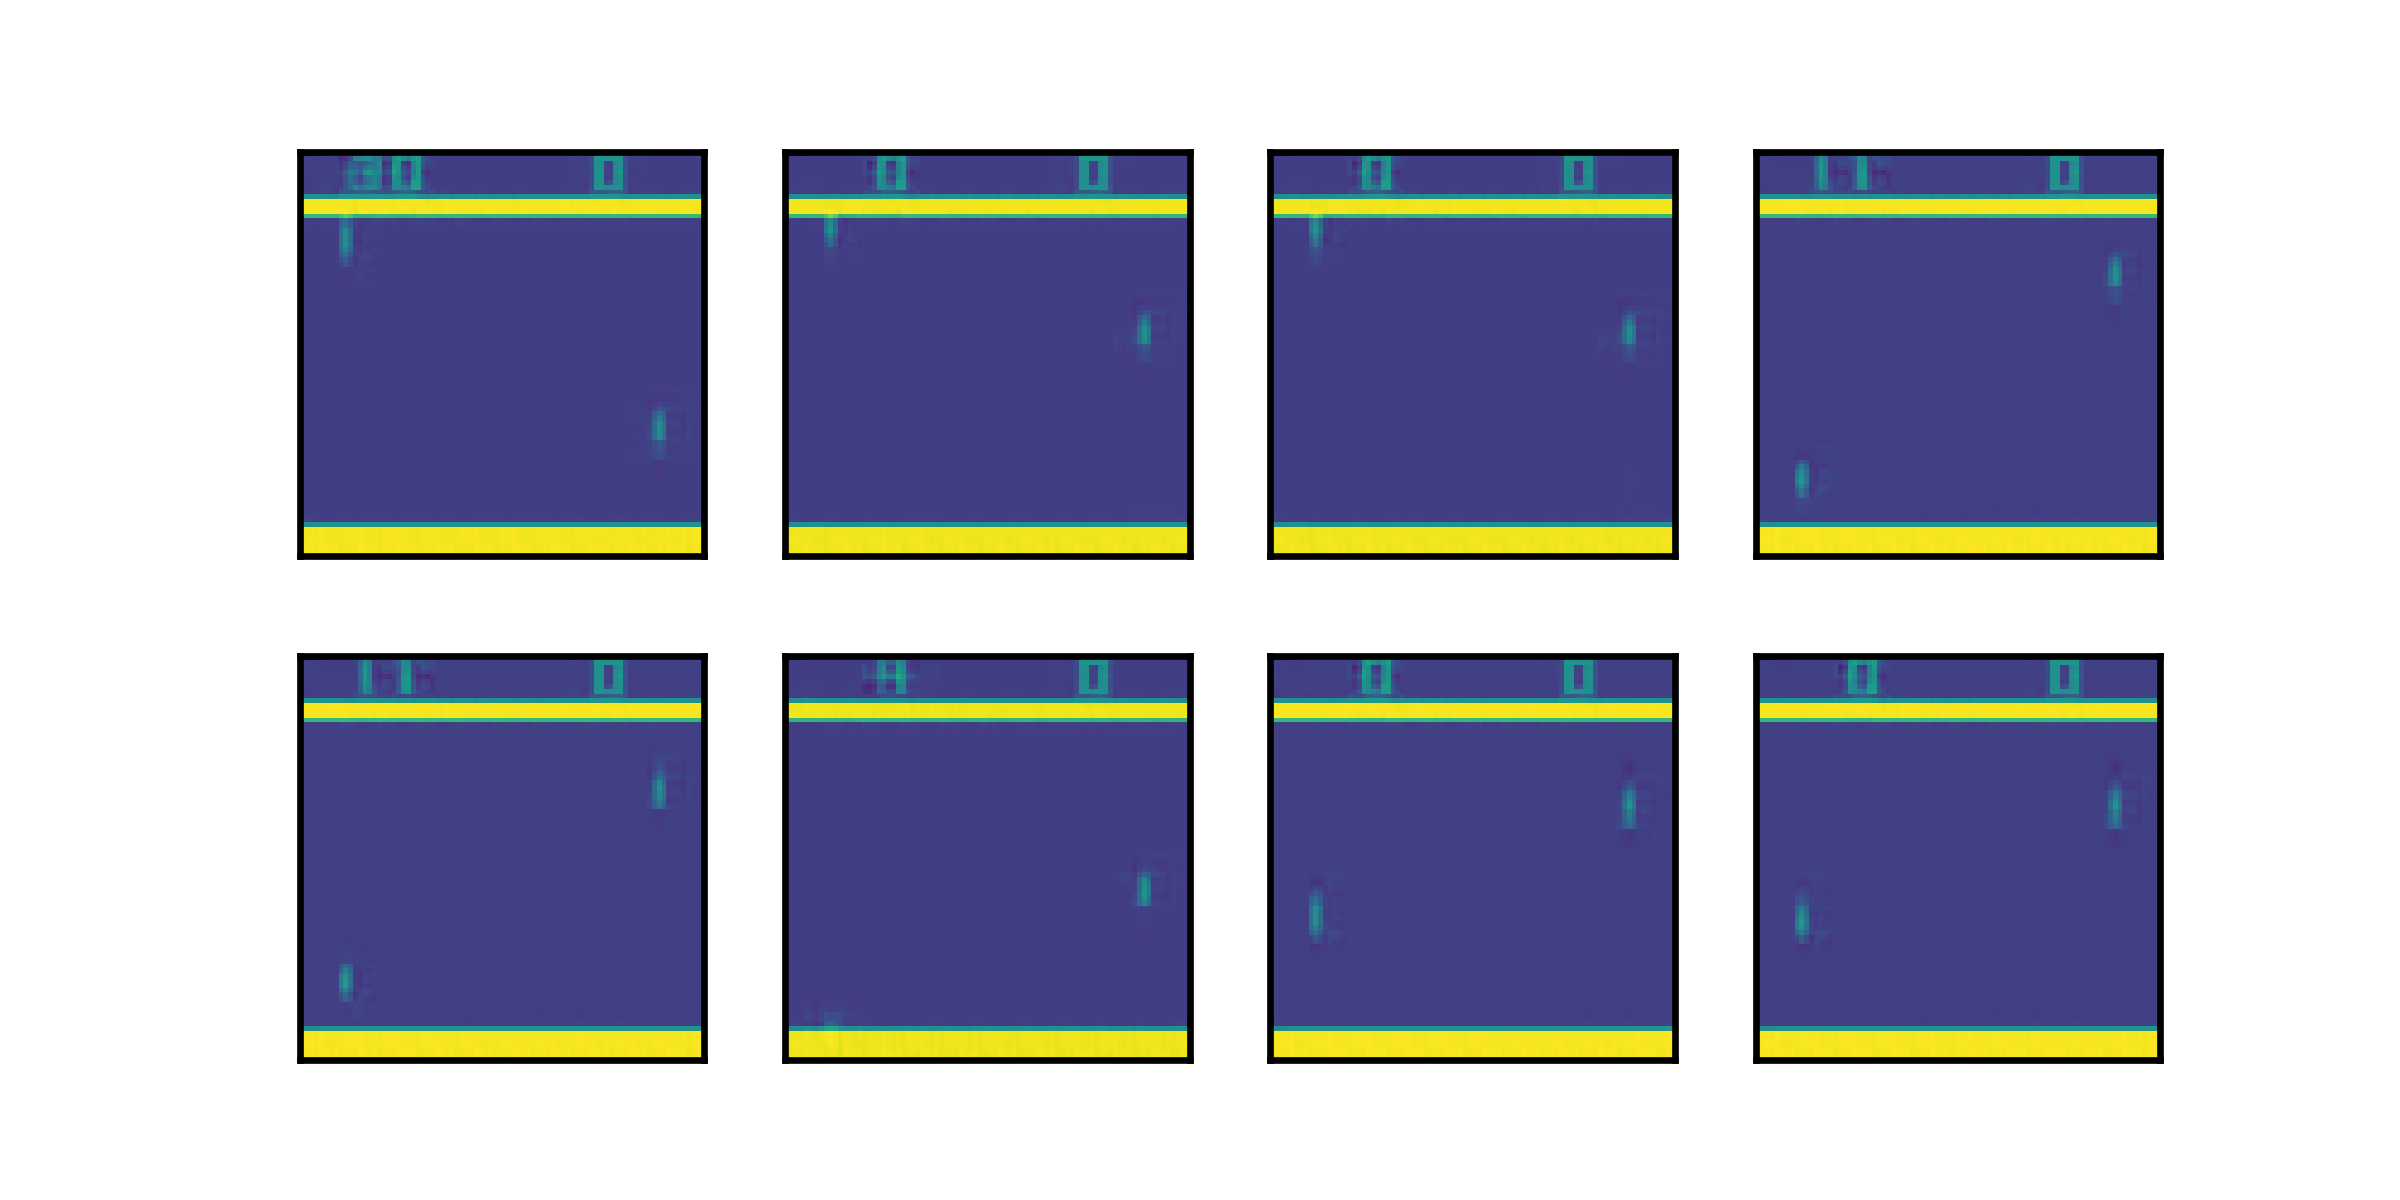
\includegraphics[width=1.0\textwidth]{../../latent_only/ae_resulting_images_features_dim_288_slightly_bigger.png}
		\caption{}
		\label{fig:}
\end{figure}



\section{Experiment}
The following network:
\begin{minted}[mathescape, linenos]{python}
if self._features_dim ==576 
    self.encoder = nn.Sequential(
        nn.Conv2d(n_input_channels, 64, kernel_size=8, stride=4, padding=0),
        nn.ReLU(),
        nn.Conv2d(64, 64, kernel_size=8, stride=2, padding=0),
        nn.ReLU(),
        nn.Conv2d(64, 64, kernel_size=4, stride=1, padding=0),
        nn.ReLU(),
        nn.Conv2d(64, 64, kernel_size=2, stride=1, padding=0),
        nn.ReLU(),
        nn.Flatten(),
    )

\end{minted}

Tried ones with less channel, but with the same feature dim, they looked like they could 
are close to working.
They ate the ball sometimes which was unacceptable.
This is should be good.

It worked, but only partially --- it worked for the data it had the most,
and 50\% of the time for data that was rarer in the dataset.


\section{Experiment}
Use the autoencoder you've pretrained.
Chop of the decoder and let the encoder be the feature portion of the Q-network.
Once that's initialized, run DQN as normal, hopefully this will result in faster learning.

\section{Experiment}
Make the autoencoder learn in parallel with the policy.
\paragraph{Why this probably won't work}
If you think about it, you're constantly changing the feature space.
And the value iteration gradienst have practically nothing to do with it.
So even if the Q network works perfectly, it won't work because the same 
frame will be encoded differently because the embedding network changed.
In a different world, gradients on new frames won't change the whole network,
but this is not the world we're living in.
If that was the case, catastrophic forgetting wouldn't be a thing.
People are trying to combat this, there's probably a paper or two to be read about this.

\paragraph{But we still have to try to and test} because this is machine learning,
and you don't really know anything and so you need to perform empiric measurements...




\section{TODO: Experiment}
The ball thing gets one thinking.
It's clearly important, despite the fact that it's a few pixels.
If you add more layers to make it reconstruct correctly, 
you also make reconstructing the score on the top of the screen more correct. 
And you don't care about that, you get the reward signal anyway.
So MSE loss (or whatever reconstruction loss) is clearly not what you actually want.

So let's train an inverse model to predict an action based on two consequtive frames,
chop some heads off (or something) and use that as the feature space --- 
that way you only train what you care about, which hopefully
means you get away with a smaller feature space,
and that's what we're after here.

When the policy or Q-network extract features, they extract features that are relevant 
for the task --- our embedding should do the same.

\end{document}
